\iffalse
Come già anticipato PICAT è un linguaggio multiparadigma, ed è stato influenzato da differenti linguaggi, sopratutto da Prolog. Inoltre è stato modellato come un linguaggi di scripting, prendendo anche come esempio Python.
\fi

\begin{frame}{Molte influenze}

	Implementa differenti paradigmi di programmazione
	\begin{itemize}
		\item Programmazione logica
		\item Programmazione imperativa
		\item Programmazione funzionale
	\end{itemize}

	\vspace{1em}
	Pensato come linguaggio di scripting

	\begin{figure}
		\centering
		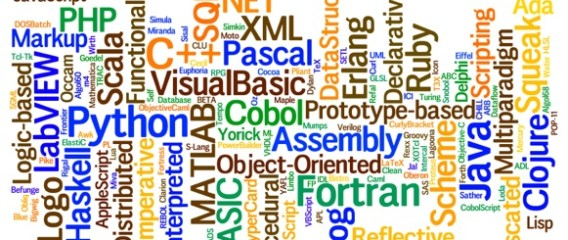
\includegraphics[scale=0.4]{res/influenze}
	\end{figure}
\end{frame}